\section{マルチラベル推定}
レスキュー犬訓練データセットのマルチラベル推定を行なった.動画で見たデータセットの前半70\%を学習、後半30\%を評価に用いた.
モデル毎にそれぞれチューニングを行い,モデル内で最も精度の良いものを示す.
各表ではクラス毎の精度と全体を合計しての精度をPrecision(適合性),Recall(再現率),Jaccard係数で示している.
なお,Jaccard係数とは\[tfrac{TP}{FP+FN+TP}\]で表され,PrecisionとRecallの両者についてF尺度と比較してより厳格な値が求まる.
レスキュー犬の行動分類にあたり,PrecisionとRecallを共に重視するためにこの係数を採用した.
よって,本研究ではJaccard係数がより大きいモデルは精度がより良いと表現する.

\subsection{静止画像からのマルチクラス推定}
静止画像からのマルチクラス推定では,ImageNetで学習したVGG16のpretrained modelを用いてのfinetuningを行なった.
推定精度を表~\ref{still_result}に示す.
%表~\ref{cyberdataset_label}と照らしあわせると,データ数の少ないものは精度が低い傾向にある.
%eatクラス,runクラスが特にその傾向を反映している.傾向とは異なるものとして,

eatクラス,runクラスが特に精度が低く,データ数の少なさと関係していると考察できる.
データ数が少ないにも関わらずPrecisionの高いshakeクラス,反対にデータ数が十分にも関わらず精度の低いsniffクラスからは,図~\ref{cyberdataset_img}に示したように画像特徴の取りやすさ、取りにくさに依存していることが確認できる.
\begin{table}[tb]
 \centering
 \caption{静止画像を用いたVGG16のfinetuning結果}\label{still_result}
 \scalebox{0.95}[1.00]{
  \begin{tabular}{|l||c|c|c|c|c|c|c|c|c|c|c|c|}
   \hline \hline
   クラス   & \rotatebox{90}{bark}& \rotatebox{90}{cling}&\rotatebox{90}{command}& \rotatebox{90}{eat}&\rotatebox{90}{handler}& \rotatebox{90}{run}&\rotatebox{90}{victim}& \rotatebox{90}{shake}& \rotatebox{90}{sniff}& \rotatebox{90}{stop}& \rotatebox{90}{walk} & \rotatebox{90}{全体}\\ \hline
Precision & 0.626& 0.112& 0.046& 0.23& 0.249& nan& 0.347& 0.896& 0.0& 0.777& 0.602&  0.576 \\ \hline
Recall    & 0.363& 0.227& 0.067& 0.031& 0.027& 0.0& 0.38& 0.3& 0.0& 0.704& 0.753&  0.605 \\ \hline
Jaccard   & 0.299& 0.081& 0.028& 0.028& 0.025& 0.0& 0.222& 0.29& 0.0& 0.586& 0.503&  0.418 \\ \hline

   % seven80_6fps_still_bc-32_lr-0_sr-5_sp-30
%   Precision & 0.643& 0.099& 0.046& 0.227& 0.226& nan& 0.333& 1.0& 0.0& 0.777& 0.602&  0.565 \\ \hline
%   Recall & 0.357& 0.227& 0.067& 0.031& 0.026& 0.0& 0.396& 0.25& 0.0& 0.71& 0.752&  0.615 \\ \hline
%   Jaccard & 0.298& 0.074& 0.028& 0.028& 0.024& 0.0& 0.221& 0.25& 0.0& 0.59& 0.503&  0.418 \\ \hline
  \end{tabular}
 }
\end{table}

\subsection{optical flow画像からのマルチクラス推定}
optical flow画像からのマルチクラス推定では,静止画像からのマルチラベル推定と同じようにImageNetで学習したVGG16のpretrained modelを用いてのfinetuningを行なった.
推定精度を表~\ref{optic_result}に示す.

静止画像と比較して,shakeクラス,stopクラスなどの動き特徴の現れやすそうなクラスの精度が高くなることを期待していたが,それらを含め全体的に精度が下がった.
画像特徴が失われたため,推定が困難になった様子がうかがえる.
\begin{table}[tb]
 \centering
 \caption{optical flow画像を用いたVGG16のfinetuning結果}\label{optic_result}
 \scalebox{0.95}[1.00]{
  \begin{tabular}{|l||c|c|c|c|c|c|c|c|c|c|c|c|}
   \hline \hline
   クラス   & \rotatebox{90}{bark}& \rotatebox{90}{cling}&\rotatebox{90}{command}& \rotatebox{90}{eat}&\rotatebox{90}{handler}& \rotatebox{90}{run}&\rotatebox{90}{victim}& \rotatebox{90}{shake}& \rotatebox{90}{sniff}& \rotatebox{90}{stop}& \rotatebox{90}{walk} & \rotatebox{90}{全体}\\ \hline
   Precision & 0.54& 0.027& 0.017& 0.183& 0.239& nan& 0.166& 0.787& 0.0& 0.761& 0.537&  0.462 \\ \hline
   Recall    & 0.198& 0.052& 0.011& 0.007& 0.042& 0.0& 0.121& 0.185& 0.0& 0.64& 0.719&  0.578 \\ \hline
   Jaccard   & 0.17& 0.018& 0.007& 0.007& 0.037& 0.0& 0.075& 0.176& 0.0& 0.533& 0.444&  0.345 \\ \hline


   % seven80_6fps_optic_bc-32_lr-0
%   Precision & 0.487& 0.048& 0.062& 0.188& 0.25& nan& 0.224& 1.0& 0.0& 0.76& 0.527&  0.53 \\ \hline
%   Recall & 0.247& 0.121& 0.044& 0.019& 0.044& 0.0& 0.171& 0.05& 0.0& 0.708& 0.705&  0.572 \\ \hline
%   Jaccard & 0.196& 0.035& 0.027& 0.017& 0.039& 0.0& 0.107& 0.05& 0.0& 0.579& 0.432&  0.38 \\ \hline
  \end{tabular}
 }
\end{table}

%\begin{figure}[htbp]
% \begin{center}
%  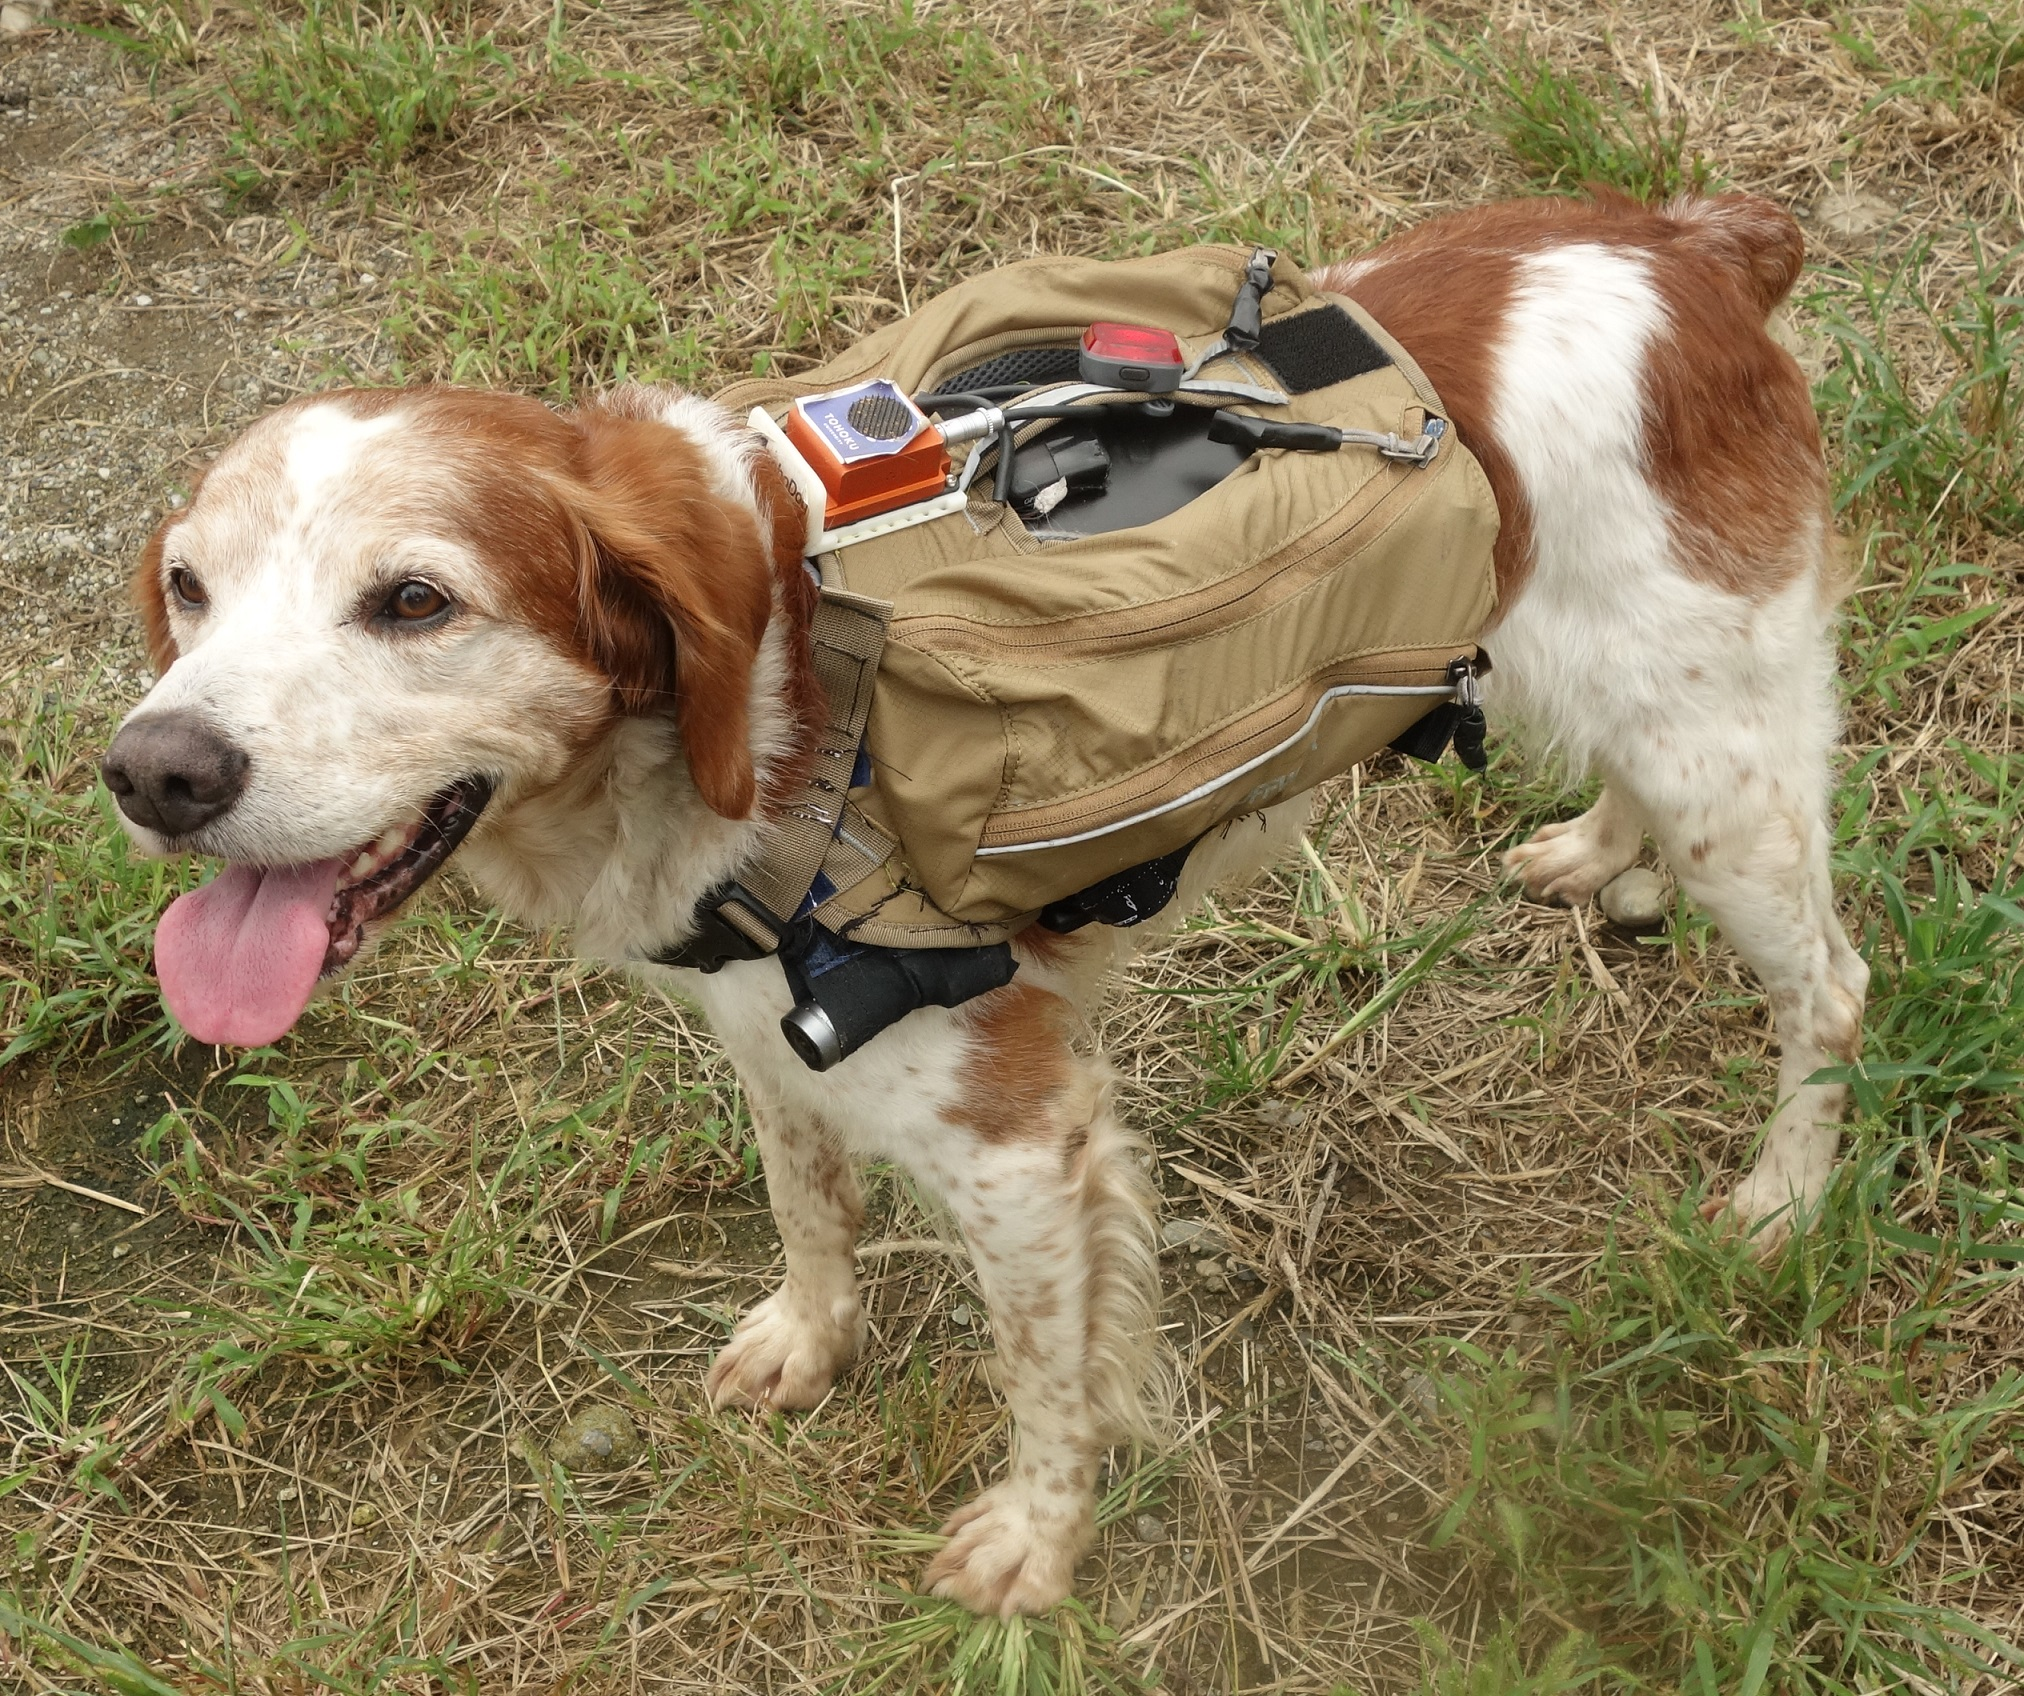
\includegraphics[width=9cm]{./Figures/cyberdog.eps}
%  \caption{装着型計測・記録装置~\cite{dog01}より引用}
%  \label{cyberdog}
% \end{center}
%\end{figure}

\subsection{音声からのマルチクラス推定}
動画の音声データのみを用いてマルチクラス推定を行なった.
ネットワークは\cite{aytar2016soundnet}の音声分類ネットワークを参考に構成した.
メル周波数スペクトラム係数を用いて音声データから特徴を取り出し,その値をネットワークへの入力とした.
29.97fpsの動画31フレーム分の音声を48000Hzとして扱い,(20, 94)次元の入力を得た.
\subsubsection{1D Convolutional network}
図~\ref{sound_network}に示したネットワークの2D Convolutionレイヤを1D Convolutionレイヤに置き換えたネットワークを用いて推定を行なった.
推定制度を表~\ref{sound_1d_result}に示す.

全体を通して,静止画像からのマルチクラス推定よりも精度が上昇した.
特に,barkクラス,commandクラス,shakeクラス,sniffクラスの精度上昇が顕著であり,音特徴がクラス推定に重要であることが示された.
\begin{table}[tb]
 \centering
 \caption{音声データを用いた1d Convolutional networkの推定結果}\label{sound_1d_result}
 \scalebox{0.95}[1.00]{
  \begin{tabular}{|l||c|c|c|c|c|c|c|c|c|c|c|c|}
   \hline \hline
   クラス   & \rotatebox{90}{bark}& \rotatebox{90}{cling}&\rotatebox{90}{command}& \rotatebox{90}{eat}&\rotatebox{90}{handler}& \rotatebox{90}{run}&\rotatebox{90}{victim}& \rotatebox{90}{shake}& \rotatebox{90}{sniff}& \rotatebox{90}{stop}& \rotatebox{90}{walk} & \rotatebox{90}{全体}\\ \hline

Precision & 0.916& 0.073& 0.345& 0.074& 0.268& 0.0& 0.294& 0.645& 0.546& 0.871& 0.77&  0.665 \\ \hline
Recall    & 0.704& 0.144& 0.362& 0.025& 0.203& 0.0& 0.338& 0.448& 0.799& 0.819& 0.893&  0.652 \\ \hline
Jaccard   & 0.661& 0.051& 0.215& 0.019& 0.131& 0.0& 0.187& 0.359& 0.48& 0.731& 0.705&  0.491 \\ \hline

   % seven80_6fps_sound_1d_bc-64_lr-4
%   Precision & 0.939& 0.129& 0.381& 0.167& 0.226& 0.0& 0.493& 0.723& 0.571& 0.91& 0.766&  0.684 \\ \hline
%   Recall    & 0.645& 0.182& 0.4& 0.028& 0.277& 0.0& 0.409& 0.54& 0.797& 0.832& 0.9&  0.665 \\ \hllne
%   Jaccard   & 0.619& 0.082& 0.243& 0.025& 0.142& 0.0& 0.288& 0.447& 0.499& 0.769& 0.706&  0.509 \\ \hline

  \end{tabular}
 }
\end{table}

\subsubsection{2D Convolutional network}
音声データから得た(20, 94)次元の入力にチャネルを追加し,(20, 94, 1)の画像としてネットワークへ入力した.
1D Convolutional networkと比較し特徴量が増え,精度がわずかに上昇した.
推定精度を表~\ref{sound_2d_label}に示す.

全体としての精度は上昇したものの,クラス別に比較した際に1D Convolutional networkで学習したモデルに劣るクラスが半数近くを占める.
学習コストなどを含めるなど評価指標を変えた際には2D Convolutional networkが劣る可能性がある.
\begin{table}[tb]
 \centering
 \caption{音声データを用いた1d Convolutional networkの推定結果}\label{sound_2d_result}
 \scalebox{0.95}[1.00]{
  \begin{tabular}{|l||c|c|c|c|c|c|c|c|c|c|c|c|}
   \hline \hline
   クラス   & \rotatebox{90}{bark}& \rotatebox{90}{cling}&\rotatebox{90}{command}& \rotatebox{90}{eat}&\rotatebox{90}{handler}& \rotatebox{90}{run}&\rotatebox{90}{victim}& \rotatebox{90}{shake}& \rotatebox{90}{sniff}& \rotatebox{90}{stop}& \rotatebox{90}{walk} & \rotatebox{90}{全体}\\ \hline
Precision & 0.844& 0.094& 0.357& 0.013& 0.192& nan& 0.407& 0.794& 0.588& 0.917& 0.808&  0.639 \\ \hline
Recall    & 0.628& 0.064& 0.285& 0.002& 0.079& 0.0& 0.284& 0.33& 0.83& 0.797& 0.898&  0.721 \\ \hline
Jaccard   & 0.563& 0.04& 0.188& 0.001& 0.059& 0.0& 0.201& 0.304& 0.524& 0.744& 0.74&  0.512 \\ \hline


   % seven80_6fps_sound_bc-64_lr-0
%Precision & 0.86& 0.116& 0.243& 0.032& 0.194& 0.0& 0.375& 0.733& 0.565& 0.909& 0.766&  0.65 \\ \hline
   %Recall & 0.754& 0.333& 0.226& 0.006& 0.128& 0.0& 0.48& 0.524& 0.824& 0.742& 0.867&  0.642 \\ \hline
   %Jaccard & 0.672& 0.094& 0.133& 0.005& 0.083& 0.0& 0.267& 0.44& 0.504& 0.691& 0.686&  0.477 \\ \hline

  \end{tabular}
 }
\end{table}

\subsection{Two-stream network}
静止画像とoptical flow画像を学習していないVGG16ネットワークにそれぞれ入力し,得られた2つの出力を結合した結果からマルチクラス推定を行なった.
推定結果を表~\ref{stilloptic_result}に示す.

静止画像単体,optical flow画像単体からの推定と比較して精度がわずかに上昇している.
特にsniffクラスなどが劇的に精度が上昇している.動画から得られた静止画像の画像特徴に加えて,optical flowから得られる動き特徴をそれぞれ用いた学習ができていると考えられる.
ただし,shakeクラスなど,静止画像とoptical flow画像がお互いに悪影響を与え全く分類できなくなってしまったクラスも存在している.
\begin{table}[tb]
 \centering
 \caption{Two-stream networkの推定結果}\label{stilloptic_result}
 \scalebox{0.95}[1.00]{
  \begin{tabular}{|l||c|c|c|c|c|c|c|c|c|c|c|c|}
   \hline \hline
   クラス   & \rotatebox{90}{bark}& \rotatebox{90}{cling}&\rotatebox{90}{command}& \rotatebox{90}{eat}&\rotatebox{90}{handler}& \rotatebox{90}{run}&\rotatebox{90}{victim}& \rotatebox{90}{shake}& \rotatebox{90}{sniff}& \rotatebox{90}{stop}& \rotatebox{90}{walk} & \rotatebox{90}{全体}\\ \hline
Precision & 0.522& 0.04& 0.315& 0.0& 0.395& nan& 0.478& nan& 0.472& 0.848& 0.771&  0.571 \\ \hline
Recall    & 0.122& 0.033& 0.047& 0.0& 0.204& 0.0& 0.36& 0.0& 0.813& 0.807& 0.833&  0.646 \\ \hline
Jaccard   & 0.11& 0.018& 0.043& 0.0& 0.155& 0.0& 0.259& 0.0& 0.426& 0.705& 0.668&  0.435 \\ \hline

   % seven80_6fps_stilloptic_bc-128_lr-0_sr-5_sp-20

  \end{tabular}
 }
\end{table}

\subsection{Sound based Two-stream network}
音声データに静止画像,optical flow画像を個別に組み合わせ,マルチクラス推定を行なった.
音声の特徴を取り出すネットワークには2D Convolutional networkを用いた.
\subsubsection{音声データと静止画像からのマルチクラス推定}
音声と静止画像を組み合わせたマルチクラス推定の結果を表~\ref{stillsound_result}に示す.
\begin{table}[tb]
 \centering
 \caption{音声と静止画像からのマルチクラス推定結果}\label{stillsound_result}
 \scalebox{0.95}[1.00]{
  \begin{tabular}{|l||c|c|c|c|c|c|c|c|c|c|c|c|}
   \hline \hline
   クラス   & \rotatebox{90}{bark}& \rotatebox{90}{cling}&\rotatebox{90}{command}& \rotatebox{90}{eat}&\rotatebox{90}{handler}& \rotatebox{90}{run}&\rotatebox{90}{victim}& \rotatebox{90}{shake}& \rotatebox{90}{sniff}& \rotatebox{90}{stop}& \rotatebox{90}{walk} & \rotatebox{90}{全体}\\ \hline
  Precision & 0.909& 0.05& 0.312& 0.051& 0.249& 0.042& 0.42& 0.56& 0.592& 0.885& 0.787&  0.661 \\ \hline
Recall    & 0.709& 0.077& 0.341& 0.028& 0.177& 0.002& 0.537& 0.589& 0.758& 0.802& 0.855&  0.673 \\ \hline
Jaccard   & 0.662& 0.031& 0.195& 0.018& 0.115& 0.002& 0.308& 0.402& 0.498& 0.726& 0.694&  0.5 \\ \hline


   %seven80_6fps_stillsound_bc-32_lr-05
  \end{tabular}
 }
\end{table}

\subsubsection{音声データとoptidcal flow画像からのマルチクラス推定}
音声とoptical flow画像を組み合わせたマルチクラス推定の結果を表~\ref{opticsound_result}に示す.
\begin{table}[tb]
 \centering
 \caption{音声とoptical flow画像からのマルチクラス推定結果}\label{opticsound_result}
 \scalebox{0.95}[1.00]{
  \begin{tabular}{|l||c|c|c|c|c|c|c|c|c|c|c|c|}
   \hline \hline
   クラス   & \rotatebox{90}{bark}& \rotatebox{90}{cling}&\rotatebox{90}{command}& \rotatebox{90}{eat}&\rotatebox{90}{handler}& \rotatebox{90}{run}&\rotatebox{90}{victim}& \rotatebox{90}{shake}& \rotatebox{90}{sniff}& \rotatebox{90}{stop}& \rotatebox{90}{walk} & \rotatebox{90}{全体}\\ \hline
Precision & 0.887& 0.071& 0.332& 0.052& 0.245& 0.143& 0.329& 0.692& 0.564& 0.881& 0.791&  0.681 \\ \hline
Recall    & 0.729& 0.177& 0.441& 0.019& 0.198& 0.01& 0.409& 0.424& 0.782& 0.845& 0.847&  0.641 \\ \hline
Jaccard   & 0.667& 0.054& 0.234& 0.014& 0.123& 0.01& 0.223& 0.356& 0.487& 0.759& 0.692&  0.493 \\ \hline

%seven80_6fps_opticsound_bc-64_lr-0
  \end{tabular}
 }
\end{table}

\subsection{Sound based Three-stream network}
表~\ref{stillopticsound_result}に示す.
\begin{table}[tb]
 \centering
 \caption{still optic sound}\label{stillopticsound_result}
 \scalebox{0.95}[1.00]{
  \begin{tabular}{|l||c|c|c|c|c|c|c|c|c|c|c|c|}
   \hline \hline
   クラス   & \rotatebox{90}{bark}& \rotatebox{90}{cling}&\rotatebox{90}{command}& \rotatebox{90}{eat}&\rotatebox{90}{handler}& \rotatebox{90}{run}&\rotatebox{90}{victim}& \rotatebox{90}{shake}& \rotatebox{90}{sniff}& \rotatebox{90}{stop}& \rotatebox{90}{walk} & \rotatebox{90}{全体}\\ \hline
Precision & 0.888& 0.165& 0.282& 0.188& 0.313& 0.212& 0.527& 0.708& 0.621& 0.891& 0.822&  0.702 \\ \hline
Recall    & 0.623& 0.423& 0.355& 0.092& 0.306& 0.029& 0.709& 0.492& 0.783& 0.861& 0.86&  0.663 \\ \hline
Jaccard   & 0.577& 0.135& 0.186& 0.066& 0.183& 0.026& 0.433& 0.409& 0.53& 0.779& 0.725&  0.518 \\ \hline


%seven80_6fps_stillopticsound_bc-128_lr-0
  \end{tabular}
 }
\end{table}
